% Define the page style
\fancypagestyle{chapterstyle}{
   \fancyhead[L]{\nouppercase{\rightmark}}
   \fancyhead[R]{Projet de fin d'études 2023-2024}
   \fancyfoot[C]{\vspace{20pt}\thepage} % Adjust the vertical space here
   \setlength{\headheight}{20pt}
   \setlength{\footskip}{30pt} % Adjust the value as needed
}

\chapter{Contexte Général}
\pagestyle{chapterstyle}
Ce chapitre met en œuvre le contexte générale du projet. Dans un premier temps, il
présente l’organisme d’accueil 4D Logiciels Maroc, son historique, sa structure, sa présence
dans le monde, ses services et son organigramme interne. Dans un deuxième temps, il décrit le contexte,
la problématique,  et les objectifs derrière le développement de ce projet. Dans
un troisième temps, il décrit la conduite du projet mettant en lumière la méthodologie
suivie et la planification à l’aide du diagramme de Gantt.



\newpage
\vspace{1cm}
% \section{Introduction}


%%%%%%%%%%%%%%%%%%%% SECTION 2 %%%%%%%%%%%%%%%%%%%%%%%

\section{Présentation de l’organisme d’accueil}
\subsection{Organisme d'accueil}

4D Logiciels, fondée en 1984 par Laurent Ribardière, est une entreprise pionnière dans
le domaine du développement d’applications professionnelles. Son objectif initial était de
simplifier la création d’applications pour les entreprises en utilisant une base de données
relationnelle entièrement graphique, une innovation favorisée par l’industrie logicielle.
\newline

En tant que l’un des premiers éditeurs de logiciels français, 
4D a étendu son rayonnement à l’échelle internationale, avec 
une présence sur les cinq continents et des filiales
dans cinq pays, y compris le Maroc


\begin{figure}[h]
    \centering
    
\includegraphics[scale=1]{Images/logo-4d.jpg} % Replace with the actual filename of the IBM logo image
    \caption{Logo 4D}
    \label{fig:Logo4D}
\end{figure}


\subsubsection{Fiche signalétique de 4D Logiciels}


\begin{table}[h!]
    \centering
    \caption{Fiche signalétique de 4D Logiciels}
    \begin{tabular}{|>{\raggedright\arraybackslash}m{6cm}|>{\raggedright\arraybackslash}m{6cm}|}
    \hline
    Création & 1984 \\ 
    \hline
    Forme juridique & Société à Responsabilité Limitée à Associé Unique \\ 
    \hline
    Secteur & Conseil et développement de logiciels. \\ 
    \hline
    Siège social & Le Pecq, France \\ 
    \hline
    Taille de l’entreprise & 200-500 employés \\ 
    \hline
    \end{tabular}
    \label{tab:fiche_signaletique}
\end{table}

%%%%%%%%%%%%%%%%%%%% subsection 1 %%%%%%%%%%%%%%%%%%%%%%%

\subsubsection{Histoire de 4D}
L’entreprise 4D a été fondée en 1984, marquant le début d’une ère d’innovation dans le
domaine des bases de données. En 1985, 4D a introduit le tout premier système de gestion
de base de données relationnelles graphiques, offrant ainsi aux entreprises une nouvelle
approche visuelle de la gestion des données. Deux ans plus tard, 4D a franchi une nouvelle
étape en lançant le premier système de gestion de base de données 32 bits, établissant
ainsi de nouveaux standards de performance et de puissance. En parallèle, 4D a étendu
sa présence en créant 4D Inc. dans la Silicon Valley en 1987, ainsi que 4D Deutschland,
GmbH en 1988, renforçant ainsi son engagement sur le marché international.


\begin{figure}[h]
    \centering
    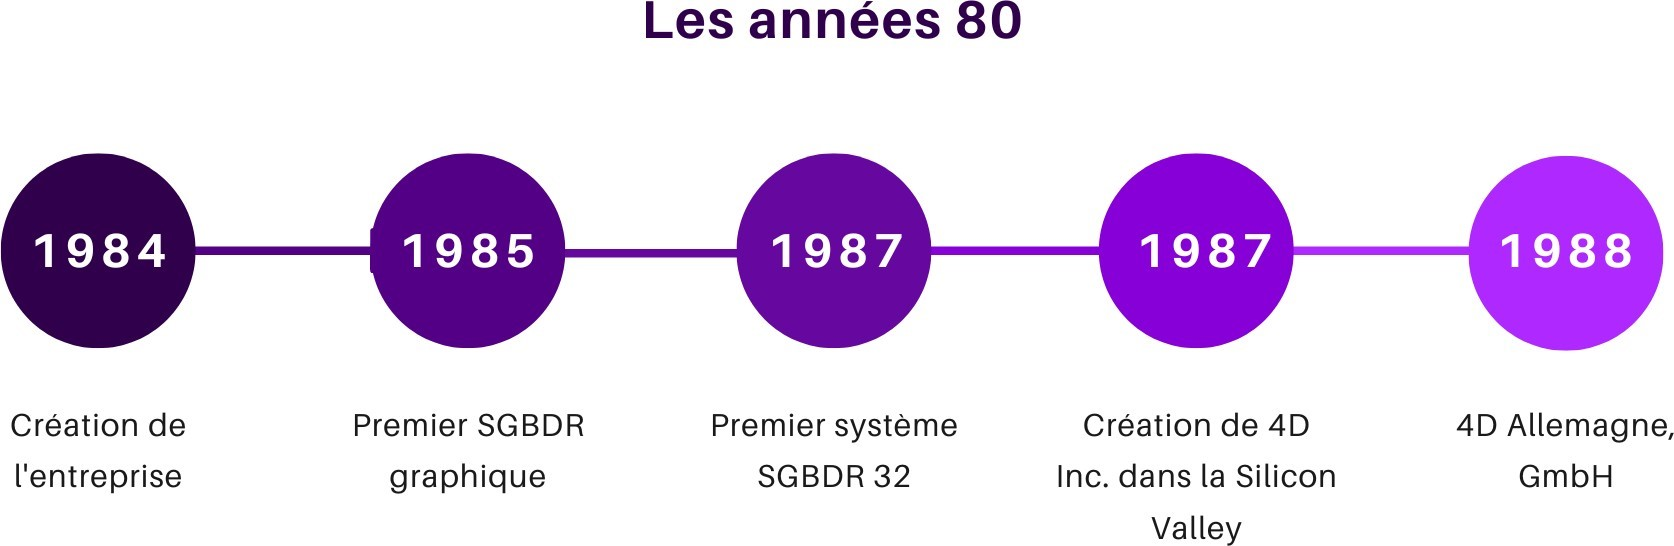
\includegraphics[scale=0.3]{Images/80.jpg} % Replace with the actual filename of the IBM logo image
    \caption{4D dans les années 80}
    \label{fig:Histoire80}
\end{figure}
\vspace{1cm}
Dans les années 90, 4D a continué d’innover en lançant en 1992 le premier système
de gestion de base de données Client/Serveur intégré. En 1995, 4D a introduit le premier
système de gestion de base de données multiplateforme, permettant aux développeurs de
créer des applications compatibles à la fois avec Mac et Windows en utilisant le même code
source. En 1997, 4D a introduit le premier système de gestion de base de données Web
dynamique, parallèlement, 4D a étendu sa présence mondiale en établissant 4D Japon en
1999, ce qui a renforcé par la suite son engagement sur le marché asiatique.
\newline

\begin{figure}[h]
    \centering
    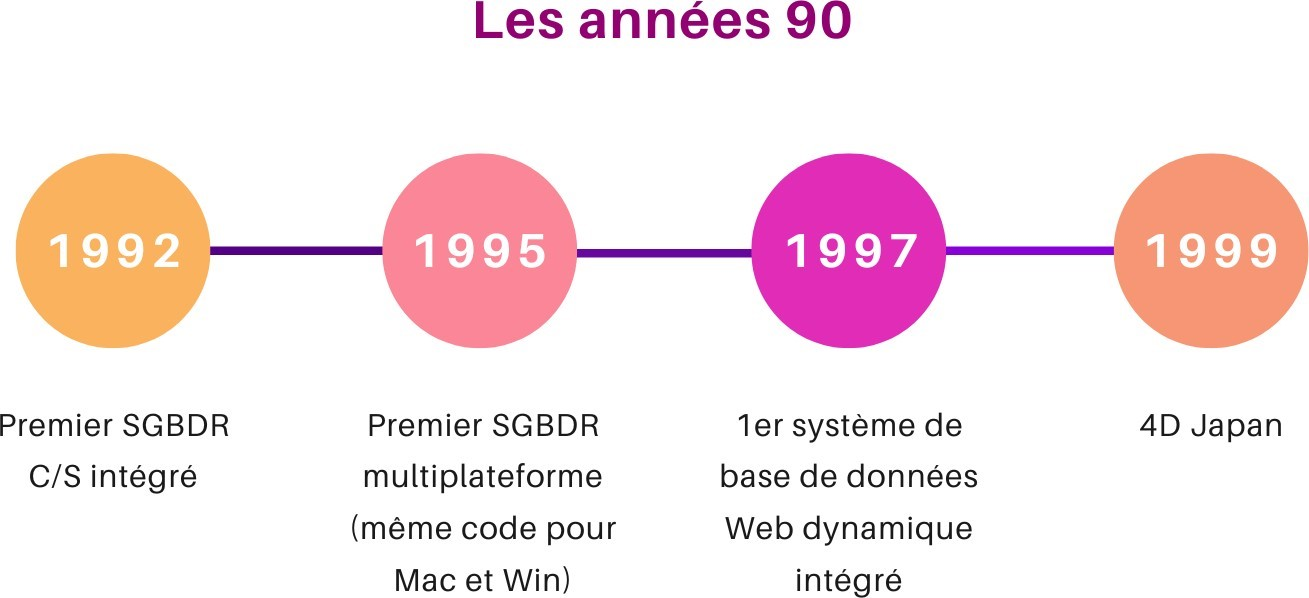
\includegraphics[scale=0.3]{Images/90.jpg} % Replace with the actual filename of the IBM logo image
    \caption{4D dans les années 90}
    \label{fig:Histoire90}
\end{figure}
% \vspace{lcm}

Ensuite, 4D Australasie Pty Ltd a été fondée en 2002, consolidant ainsi sa présence
en Australie et en Nouvelle-Zélande. En 2004, 4D a lancé la première IDE permettant de
créer des applications Client/Serveur, Web ou SOA sans avoir à modifier le code source.
En 2012, 4D a inventé la ligne de produits Wakanda, la première plateforme JavaScript de
bout en bout. En parallèle, une autre filiale a été créée au Maroc en 2012 pour renforcer
son existence sur le continent africain.
En 2016, la ligne de produits Wakanda a été reconnue par Gartner en tant que ”Cool
vendor”, confirmant ainsi l’engagement continu de 4D envers l’innovation et l’excellence
dans le domaine des technologies de développement d’applications.
\vspace{2cm}

\begin{figure}[h]
    \centering
    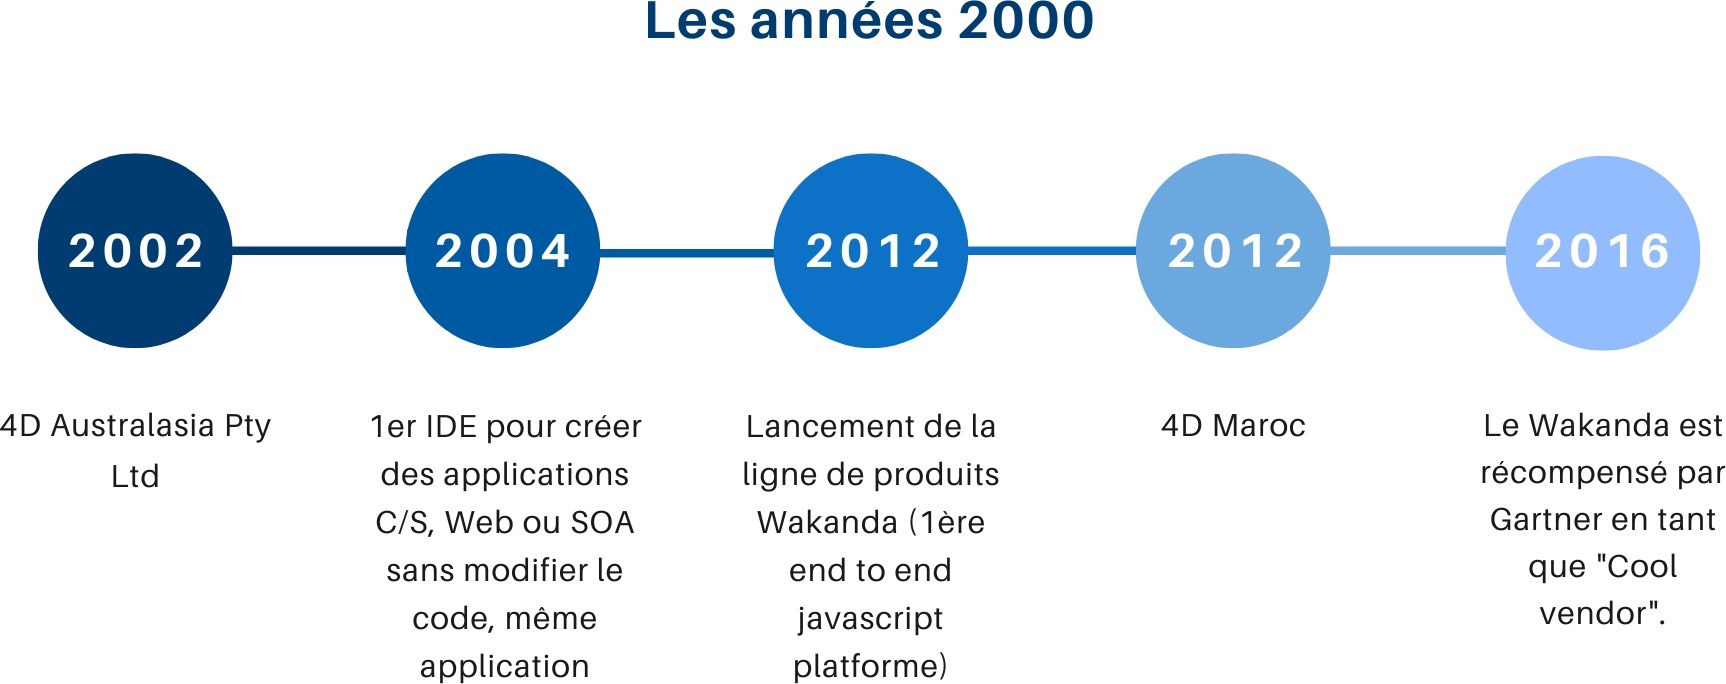
\includegraphics[scale=0.3]{Images/20.jpg} % Replace with the actual filename of the IBM logo image
    \caption{4D dans les années 2000}
    \label{fig:Histoire90}
\end{figure}


\subsection{Framework 4D}
4D est une plateforme de développement productive qui permet aux clients de se concentrer sur leur modèle de données et les règles et spécificités de leur métier. Le framework 4D prend en charge l’exécution native de leur code applicatif sous macOS et Windows. 4D Server exécute leur applications simultanément sur les postes de travail / clients mobiles et sur le Web. Ils peuvent déployer des applications entièrement personnalisées sous leur propre marque.
4D est un système de gestion de base de données relationnelle disposant d’un langage de programmation de la quatrième génération. Environnement de développement intégré, 4D intègre :
\newline

\begin{itemize}
    \item[•] un compilateur
    \item[•] un débogueur
    \item[•] un système de sauvegarde et de réplication
    \item[•] un serveur et client de services web
    \newline
\end{itemize}

 
\begin{figure}[h]
    \centering
    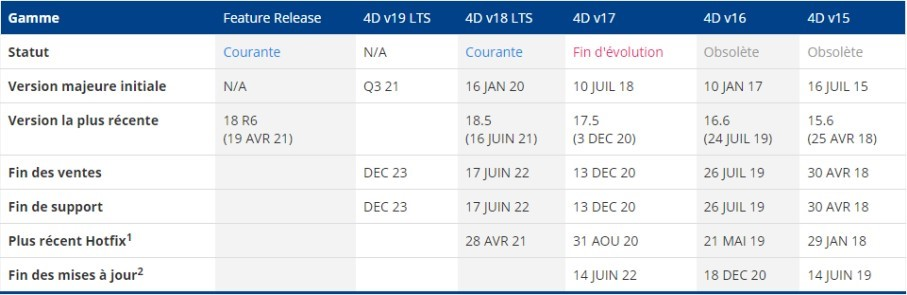
\includegraphics[scale=0.6]{Images/versions.jpg} % Replace with the actual filename of the IBM logo image
    \caption{Anciennes versions du langage 4D}
    \label{fig:Histoire90}
\end{figure}

4D v18 marque un véritable tournant dans l’histoire de 4D. 
Cette version propose non seulement de multiples nouvelles 
fonctionnalités mais aussi l’amélioration de fonctions existantes. 
Elle introduit la gestion de version pour changer la façon dont 
les équipes collaborent. Le format texte des bases projets permet 
désormais de tirer pleinement parti des systèmes de gestion de 
version (par exemple, Git, SVN, etc.). Autre fonctionnalité qui 
fait ses débuts dans cette nouvelle version : une solution intégrée
de chiffrement des données, offrant en un seul clic une sécurité
maximum aux données des clients. Ces outils de chiffrement sont
basés sur l’un des algorithmes les plus sûrs : Advanced 
Encryption Standard (AES). ORDA (Object Relational Data Access),
la technologie révolutionnaire d’accès et de présentation des 
données, apporte également son lot de nouvelles fonctionnalités,
telles que le datastore distant, ouvrant de nouvelles perspectives 
et optimisant les performances du client/serveur. Les applications métiers peuvent facilement être déployées sur des appareils mobiles avec 4D for iOS, une solution entièrement intégrée à 4D. De plus, 4D Write Pro, outil de PAO intégré à 4D, poursuit sa montée en puissance, le langage de programmation 4D s’enrichit et apporte de nouvelles commandes destinées à améliorer l’expérience de développement.


%%%%%%%%%%%%%%%%%%%% subsection 2 %%%%%%%%%%%%%%%%%%%%%%%

\subsubsection{La structure du groupe 4D}
Le groupe 4D est composé d’un siège social situé en France, et de cinq filiales situées
aux États-Unis, en Allemagne, en Australie, au Japon, et au Maroc.

% \vspace{lcm}
\begin{figure}[h]
    \centering
    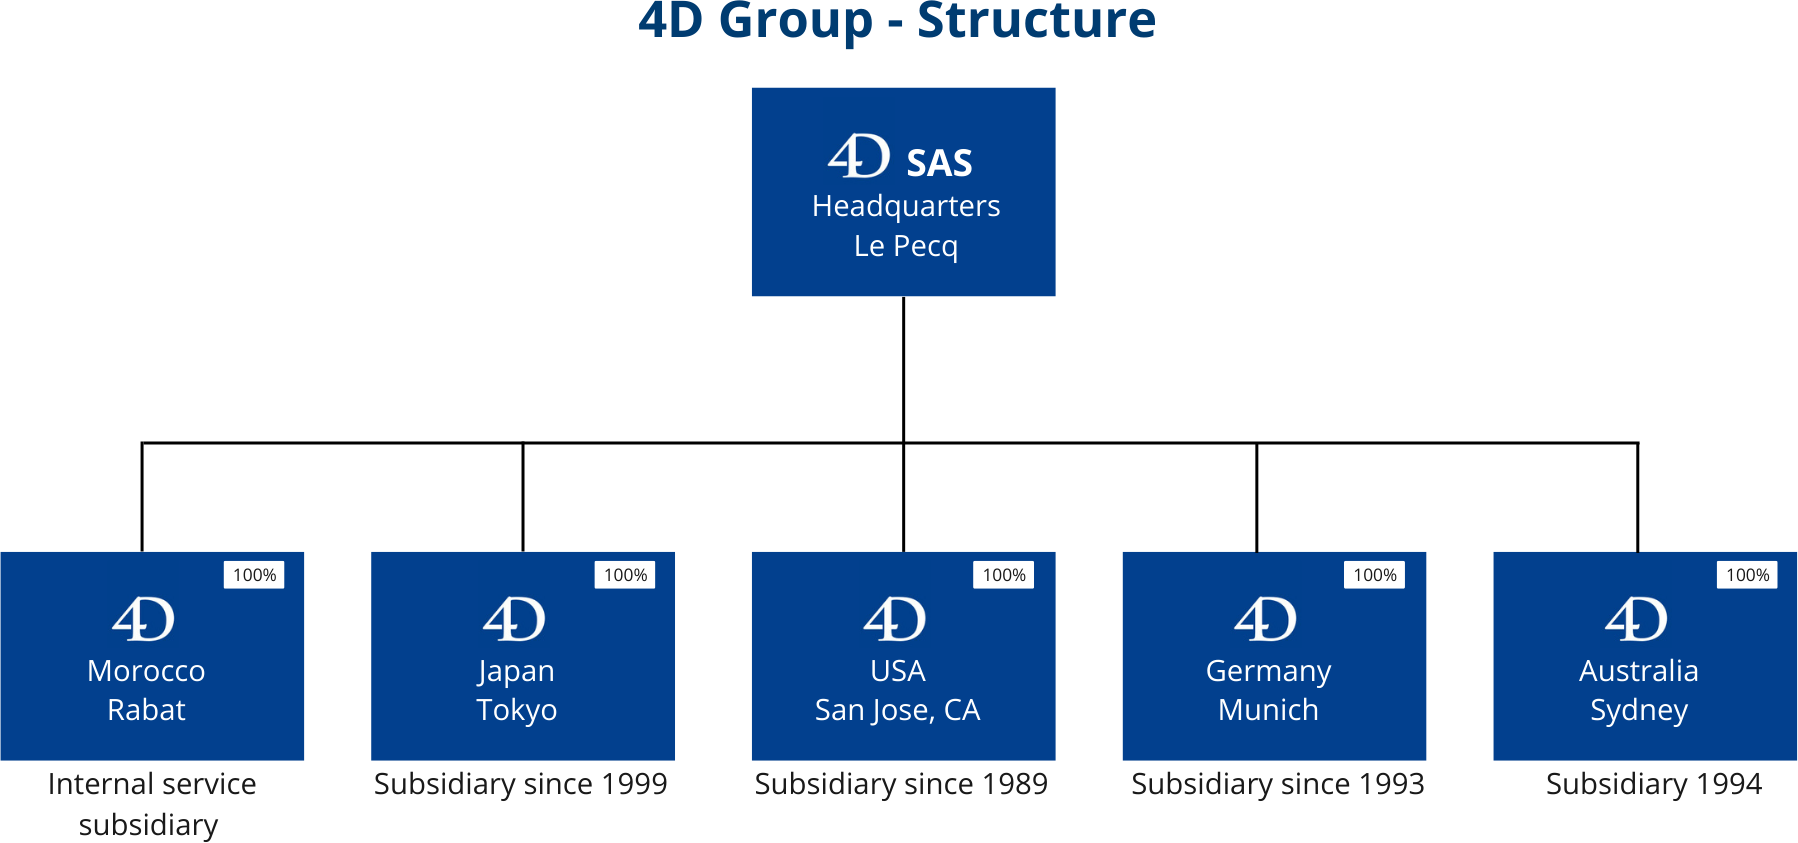
\includegraphics[scale=0.35]{Images/groupe.png} % Replace with the actual filename of the IBM logo image
    \caption{ La structure du groupe 4D}
    \label{fig:groupe}
\end{figure}

\subsubsection{Présence de 4D Logiciels dans le monde}
Comme toute société renommée, 4D recourt à ses différents partenaires pour un rendu
meilleur et un niveau d’expertise plus crédible. 4D connaît aussi une présence 
internationale grâce à ses partenaires et ses distributeurs éparpillés dans le monde, 
comme montre la figure suivante :


\begin{figure}[h]
    \centering
    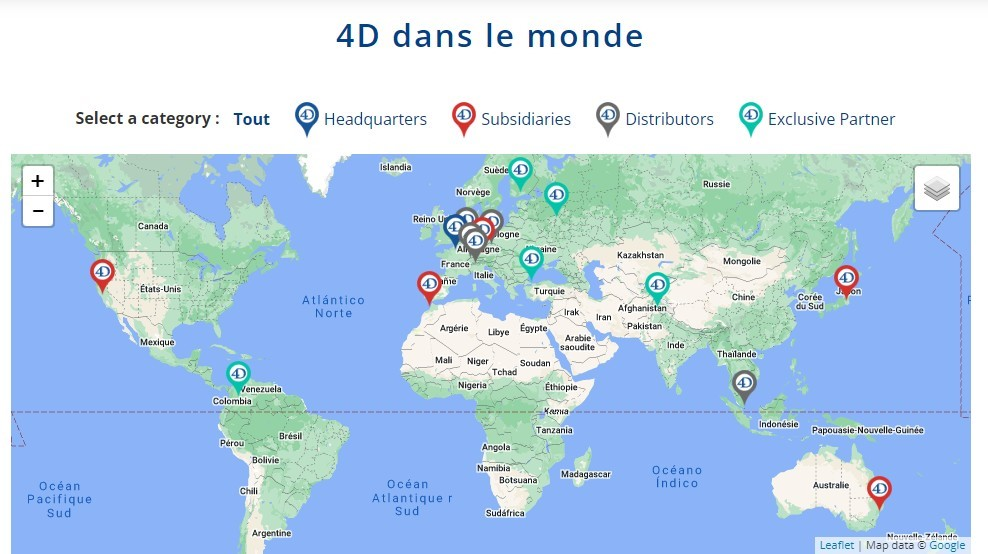
\includegraphics[scale=0.6]{Images/carte.jpg} % Replace with the actual filename of the IBM logo image
    \caption{Présence de 4D Logiciels dans le monde}
    \label{fig:carte}
\end{figure}

\vspace{3cm}

\subsubsection{Services offerts par 4D Logiciels}
4D Logiciels offre plusieurs services dans le domaine informatique, à savoir :
\\ 

\begin{itemize}
    \item[ • ] \textbf{4D Professional Services: } 4D offre une panoplie de services pour répondre aux besoins en développement logiciel, mettant à disposition une équipe qualifiée et des ressources de premier ordre à chaque étape du projet.\\
    \item[ • ] \textbf{Migration des bases de données 4D :} 4D assure une transition sans heurts des bases de données 4D vers de nouveaux environnements ou versions, garantissant l’intégrité et la compatibilité des données tout en minimisant les perturbations opérationnelles.\\
    \item[ • ] \textbf{Migration 64-Bits : } 4D assure une mise à niveau efficace des applications vers des environnements 64-bits, améliorant ainsi la performance, la stabilité et la sécurité des systèmes sans compromettre la fonctionnalité existante.\\
    \item[ • ] \textbf{Développement Mobile et Web :}  4D fournit un accompagnement expert dans la conception et le développement sur mesure d’applications mobiles et web, en mettant un accent particulier sur l’optimisation de l’expérience utilisateur et l’intégration harmonieuse avec l’infrastructure informatique.\\
    \item[ • ] \textbf{Audit de sécurité :}  4D réalise une évaluation approfondie de la sécurité des environnements informatiques, identifiant les vulnérabilités potentielles et proposant des stratégies proactives pour renforcer la protection des données et systèmes contre les menaces externes et internes.\\
    \item[ • ] \textbf{Service Assurance Qualité et Automatisation:}  4D propose un service de tests automatisés, un service d’intégration continue ainsi qu’un service de tests fonctionnels et non fonctionnels dans l’optique d’améliorer l’efficacité des processus des applications métier de ces clients.
\end{itemize}


\subsection{Organigramme de l’organisme d’accueil}
La figure ci-dessous montre la hiéararchie de la direction générale de l’entreprise 4D
logiciels :

\begin{figure}[h]
    \centering
    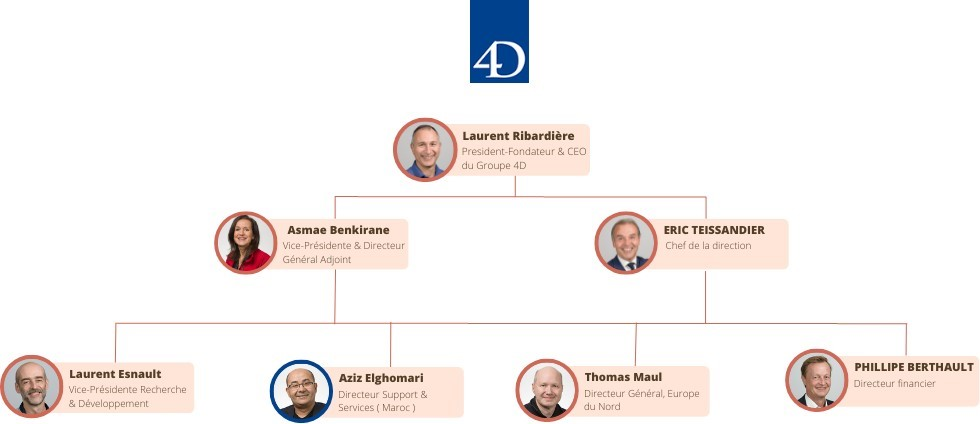
\includegraphics[scale=0.6]{Images/direction.jpg} % Replace with the actual filename of the IBM logo image
    \caption{La Direction Générale de 4D}
    \label{fig:direction}
\end{figure}


% \subsection{Cadre du projet}
% Dans un environnement où la concurrence pour attirer les meilleurs talents
%  est de plus en plus intense, les entreprises doivent disposer d'outils 
%  efficaces pour gérer leur processus de recrutement. Actuellement, 
%  4D Logiciels utilise un système disparate et manuel pour le recrutement, 
%  ce qui entraîne des inefficacités et des pertes de temps. Cette situation 
%  rend difficile la gestion des candidatures, la traçabilité des étapes de 
%  recrutement, et la communication entre les recruteurs et les candidats.

% Afin de renforcer le niveau de ses collaborateurs, 4D Logiciels souhaite 
% simplifier et moderniser son processus de recrutement. L'objectif est de passer 
% d'un système essentiellement manuel à une solution plus intégrée et automatisée, 
% permettant d'améliorer l'efficacité, de réduire les délais de recrutement, 
% et d'offrir une meilleure expérience aux candidats.

% \subsection{Problématique}
% L'entreprise 4D Logiciels est confrontée à une gestion inefficace
%  de ses processus de recrutement, notamment lorsqu'elle publie 
%  des offres d'emploi et ouvre des opportunités de stage annuelles.
% 4D Logiciels reçoit un grand nombre de candidatures non triées,
% provenant de divers domaines, ce qui rend difficile la
% sélection des candidats les plus appropriés. Les méthodes 
% traditionnelles utilisées, telles que les emails, les tableurs 
% et les calendriers, ne permettent pas de gérer efficacement 
% ce flux de candidatures. De plus, les applications de recrutement
%  disponibles sur le marché ne répondent pas pleinement aux 
%  besoins spécifiques de l'entreprise en termes de processus 
%  de recrutement.

% En considérant les défis actuels du processus de recrutement chez
%  4D Logiciels, une interrogation primordiale se profile : 
%  comment transformer efficacement le processus de recrutement 
%  afin de surmonter les obstacles liés au traitement manuel des 
%  candidatures, à la dispersion des données et à la gestion 
%  disjointe des entretiens, assurant ainsi une sélection de 
%  candidats plus optimale et équitable pour l'organisation ?


% \subsection{Les objectifs}

% Pour répondre efficacement à la problématique identifiée,
% la solution proposée doit satisfaire les objectifs suivants :

% \begin{itemize}
%     \item Centraliser et Automatiser la Gestion des Candidatures
%     \item Améliorer la Sélection des Candidats 
%     \item Optimiser la Traçabilité et la Suivi des Étapes de Recrutement 
%     \item Faciliter la Communication et la Collaboration 
%     \item Analyser et Optimiser les Performances du Processus de Recrutement 
%     \item Offrir une Meilleure Expérience Candidat 
% \end{itemize}

% %%%%%%%%%%%%%%%%%%%% SECTION 4 %%%%%%%%%%%%%%%%%%%%%%%

\section{Contexte général du projet}

\section{Cadre du projet }

% Actuellement, les processus de recrutement au sein de 4D Logiciels
% Maroc sont gérés de manière dispersée, chaque département utilise 
% sa propre méthode de recrutement. Cette fragmentation conduit à 
% des inefficacités et des difficultés de coordination. Le volume 
% élevé de candidatures et de CV reçus par mail ne peut pas être 
% traité de manière manuelle efficace, ce qui complique encore 
% davantage le suivi et la gestion des informations. En l'absence 
% d'un système centralisé, il devient impératif de moderniser et 
% de centraliser ces processus pour améliorer la cohérence et 
% l'efficacité de recrutement.
Les processus de recrutement chez 4D Logiciels Maroc sont 
actuellement fragmentés, chaque département utilisant sa propre 
méthode. Cette dispersion entraîne des inefficacités et des 
difficultés de coordination, surtout avec le volume élevé de 
candidatures et de CVs reçus par mail de divers domaines, rendant le traitement 
manuel inefficace. L'utilisation d'emails, de tableurs et de 
calendriers traditionnels complique la sélection des candidats 
appropriés. De plus, les applications de recrutement disponibles 
ne répondent pas aux besoins spécifiques de l'entreprise. Ainsi, 
il est crucial de moderniser et de centraliser ces processus 
pour améliorer la cohérence et l'efficacité du recrutement.

\subsection{Problématique}
% L'entreprise 4D Logiciels est confrontée à une gestion inefficace
%  de ses processus de recrutement, notamment lorsqu'elle publie 
%  des offres d'emploi et ouvre des opportunités de stage annuelles.
% 4D Logiciels reçoit un grand nombre de candidatures non triées,
% provenant de divers domaines, ce qui rend difficile la
% sélection des candidats les plus appropriés. Les méthodes 
% traditionnelles utilisées, telles que les emails, les tableurs 
% et les calendriers, ne permettent pas de gérer efficacement 
% ce flux de candidatures. De plus, les applications de recrutement
%  disponibles sur le marché ne répondent pas pleinement aux 
%  besoins spécifiques de l'entreprise en termes de processus 
%  de recrutement.

En considérant les défis actuels du processus de recrutement chez
 4D Logiciels, une interrogation primordiale se profile : 
 comment transformer efficacement le processus de recrutement 
 afin de surmonter les obstacles liés au traitement manuel des 
 candidatures, à la dispersion des données et à la gestion 
 disjointe des entretiens, assurant ainsi une sélection de 
 candidats plus optimale et équitable pour l'organisation ?

\subsection{Objectifs}

% Pour répondre efficacement à la problématique identifiée,
% la solution proposée doit satisfaire les objectifs suivants :

% \begin{itemize}
%     \item[•] Centraliser et automatiser la gestion des candidatures
%     \item[•] Améliorer la sélection des candidats 
%     \item[•] Optimiser la traçabilité et le suivi des étapes de recrutement 
%     \item[•] Faciliter la Communication et la Collaboration 
%     \item[•] Analyser et optimiser les performances du processus de recrutement 
%     \item[•] Offrir une meilleure expérience candidat 
% \end{itemize}

Les objectifs du projet sont de centraliser les processus de recrutement en mettant en place une plateforme unique pour coordonner toutes les étapes, 
d'automatiser le tri des candidatures à l'aide d'outils efficaces, 
et d'améliorer la gestion des informations pour assurer une 
meilleure organisation et un suivi efficace des candidatures. 
Le projet vise également à réduire les inefficacités en minimisant 
les retards et les erreurs liés aux méthodes manuelles, 
à optimiser la sélection des candidats en facilitant 
l'identification des profils les plus qualifiés, et à offrir une 
meilleure expérience utilisateur grâce à une interface intuitive 
et professionnelle. Enfin, il s'agit de développer des solutions 
personnalisées qui répondent aux besoins spécifiques de 4D 
Logiciels Maroc en matière de recrutement.

\section{Conduite de projet}
\subsection{Méthodologie suivie}
Pour mener à bien notre projet, nous avons adopté une approche hybride 
combinant des éléments de la méthode en cascade avec des incréments. 
Le projet a démarré avec un cahier des charges initial peu clair, 
mais suffisamment détaillé pour fournir une direction générale. 
Nous avons segmenté le travail en incréments, chaque itération se 
concentrant sur le développement de fonctionnalités spécifiques. 
Des réunions régulières avec mon encadrant, qui jouait le rôle de 
Product Owner, ont permis de raffiner les besoins et de réévaluer 
les priorités en fonction des retours obtenus.

\subsection{Planification}
La mise en place de la planification a été réalisée à l’aide du logiciel de gestion de
projet GanttPRO, qui simplifie la planification et la mise en œuvre des projets grâce à
l’utilisation de diagrammes de Gantt qui fournit un aperçu clair du projet, y compris les
tâches, les dates, les délais, les dépendances.
La figure ci-dessous montre la planification du projet, avec le diagramme de Gantt,
qui s’étale sur une période de quatre mois, commençant par une formation globale sur
le langage 4D et l’analyse des besoins, passant par la conception et le développement
jusqu’aux tests end to end.

\begin{figure}[h]
    \centering
    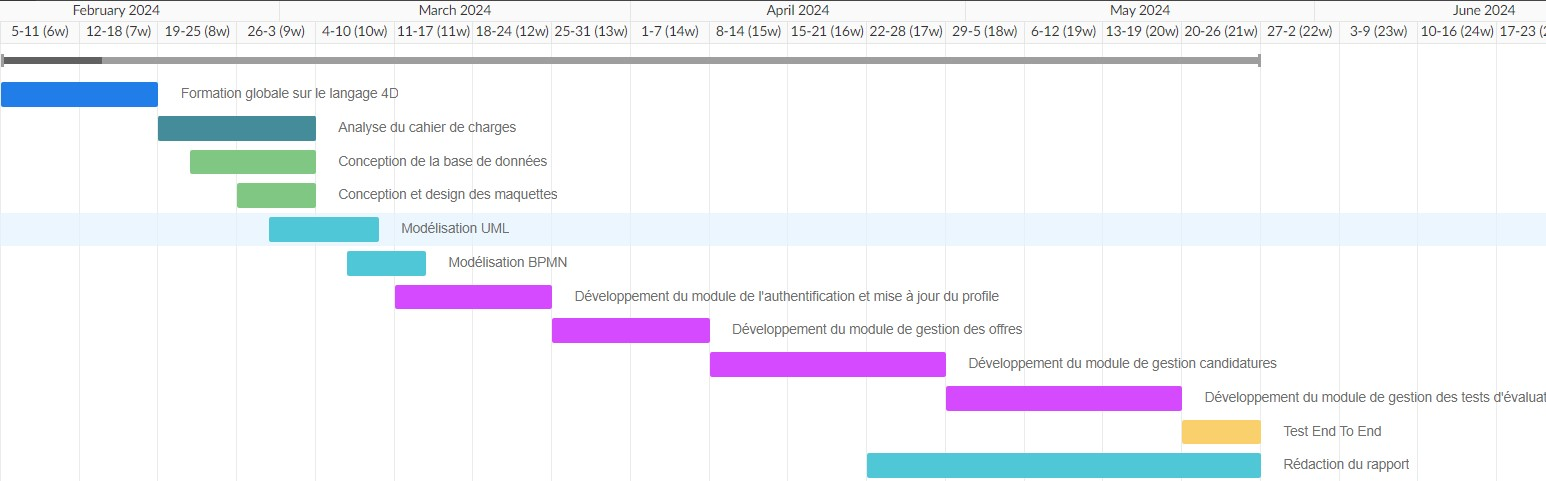
\includegraphics[scale=0.6]{Images/gantt.jpg} % Replace with the actual filename of the IBM logo image
    \caption{Diagramme de Gantt}
    \label{fig:gantt}
\end{figure}


\section{Conclusion}
En guise de conclusion, ce chapitre a élucidé les fondements de l’étude du projet
menée; en fournissant une vue d’ensemble de l’organisme d’accueil, 4D Logiciels Maroc,
et de son fonctionnement interne. Il a également exposé le cadre du projet et la problématique à laquelle
il répond, mettant en lumière les défis auxquels l’entreprise est confrontée dans son
processus de recrutement actuel, ainsi que les objectifs à accomplir. Enfin, il a établi la
démarche et la planification du projet.


